\documentclass[]{article}

\usepackage[]{graphicx}

\title{CS 636 Assignment 4: Image Classification}


\author{Derek Jones}


\begin{document}

\maketitle

\begin{abstract}
	I train a random forest and a logistic regression classifier on a random sample of 500 example images from each of the classes. I chose to try two methods in order to obtain extra credit for the assignment as well as get an idea of the performance of each with respect to the parameter of interest in my experiments, feature type while I use $k$-fold cross validation to asses how well each model can generalize.. My results show that the bag of words features, used in field such as NLP and computer vision, are suboptimal compared to the features generated by the AlexNet deep convolutional neural network. Modern advances in image classification make better use of raw image data, generating more useful features as a byproduct. 
\end{abstract}


\section{Bag of Words}

For the bag of words implementation, I aggregate a random subset of the surf features (throwing out examples in which the number of features is less than a threshold specified as a parameter in the make\_codebook() function) and then perform k-means (50 clusters, maximum of 300 iterations) to solve for the code book. Then for each of the training examples, I iterate over each surf feature and predict the cluster that the given feature belongs to. I form a histogram over all of the possible clusters, of which there are 50 total as specified in the assignment, then normalize this (as the number of features varies between examples, normalization makes this less relevant) and use this as my feature vector.

\subsection{Random Forest}

 I train a random forest classifier which is provided via the scikit-learn library with $n = 100$ decision stumps, using default settings for all other parameters. I choose this number of trees in order to decrease computation time, I've also found limited marginal gain by increasing the size of the forest (the largest I've tried is $n=100$ decision stumps). My results give a $k$-fold cross validation (on the training set, $k = 5$) average accuracy of 34.7\%. The random forest is also able to perfectly classify the full training set of 500 examples. Finally the test accuracy of this method is rather disappointing at $5.0$\%. The confusion matrix is given below:

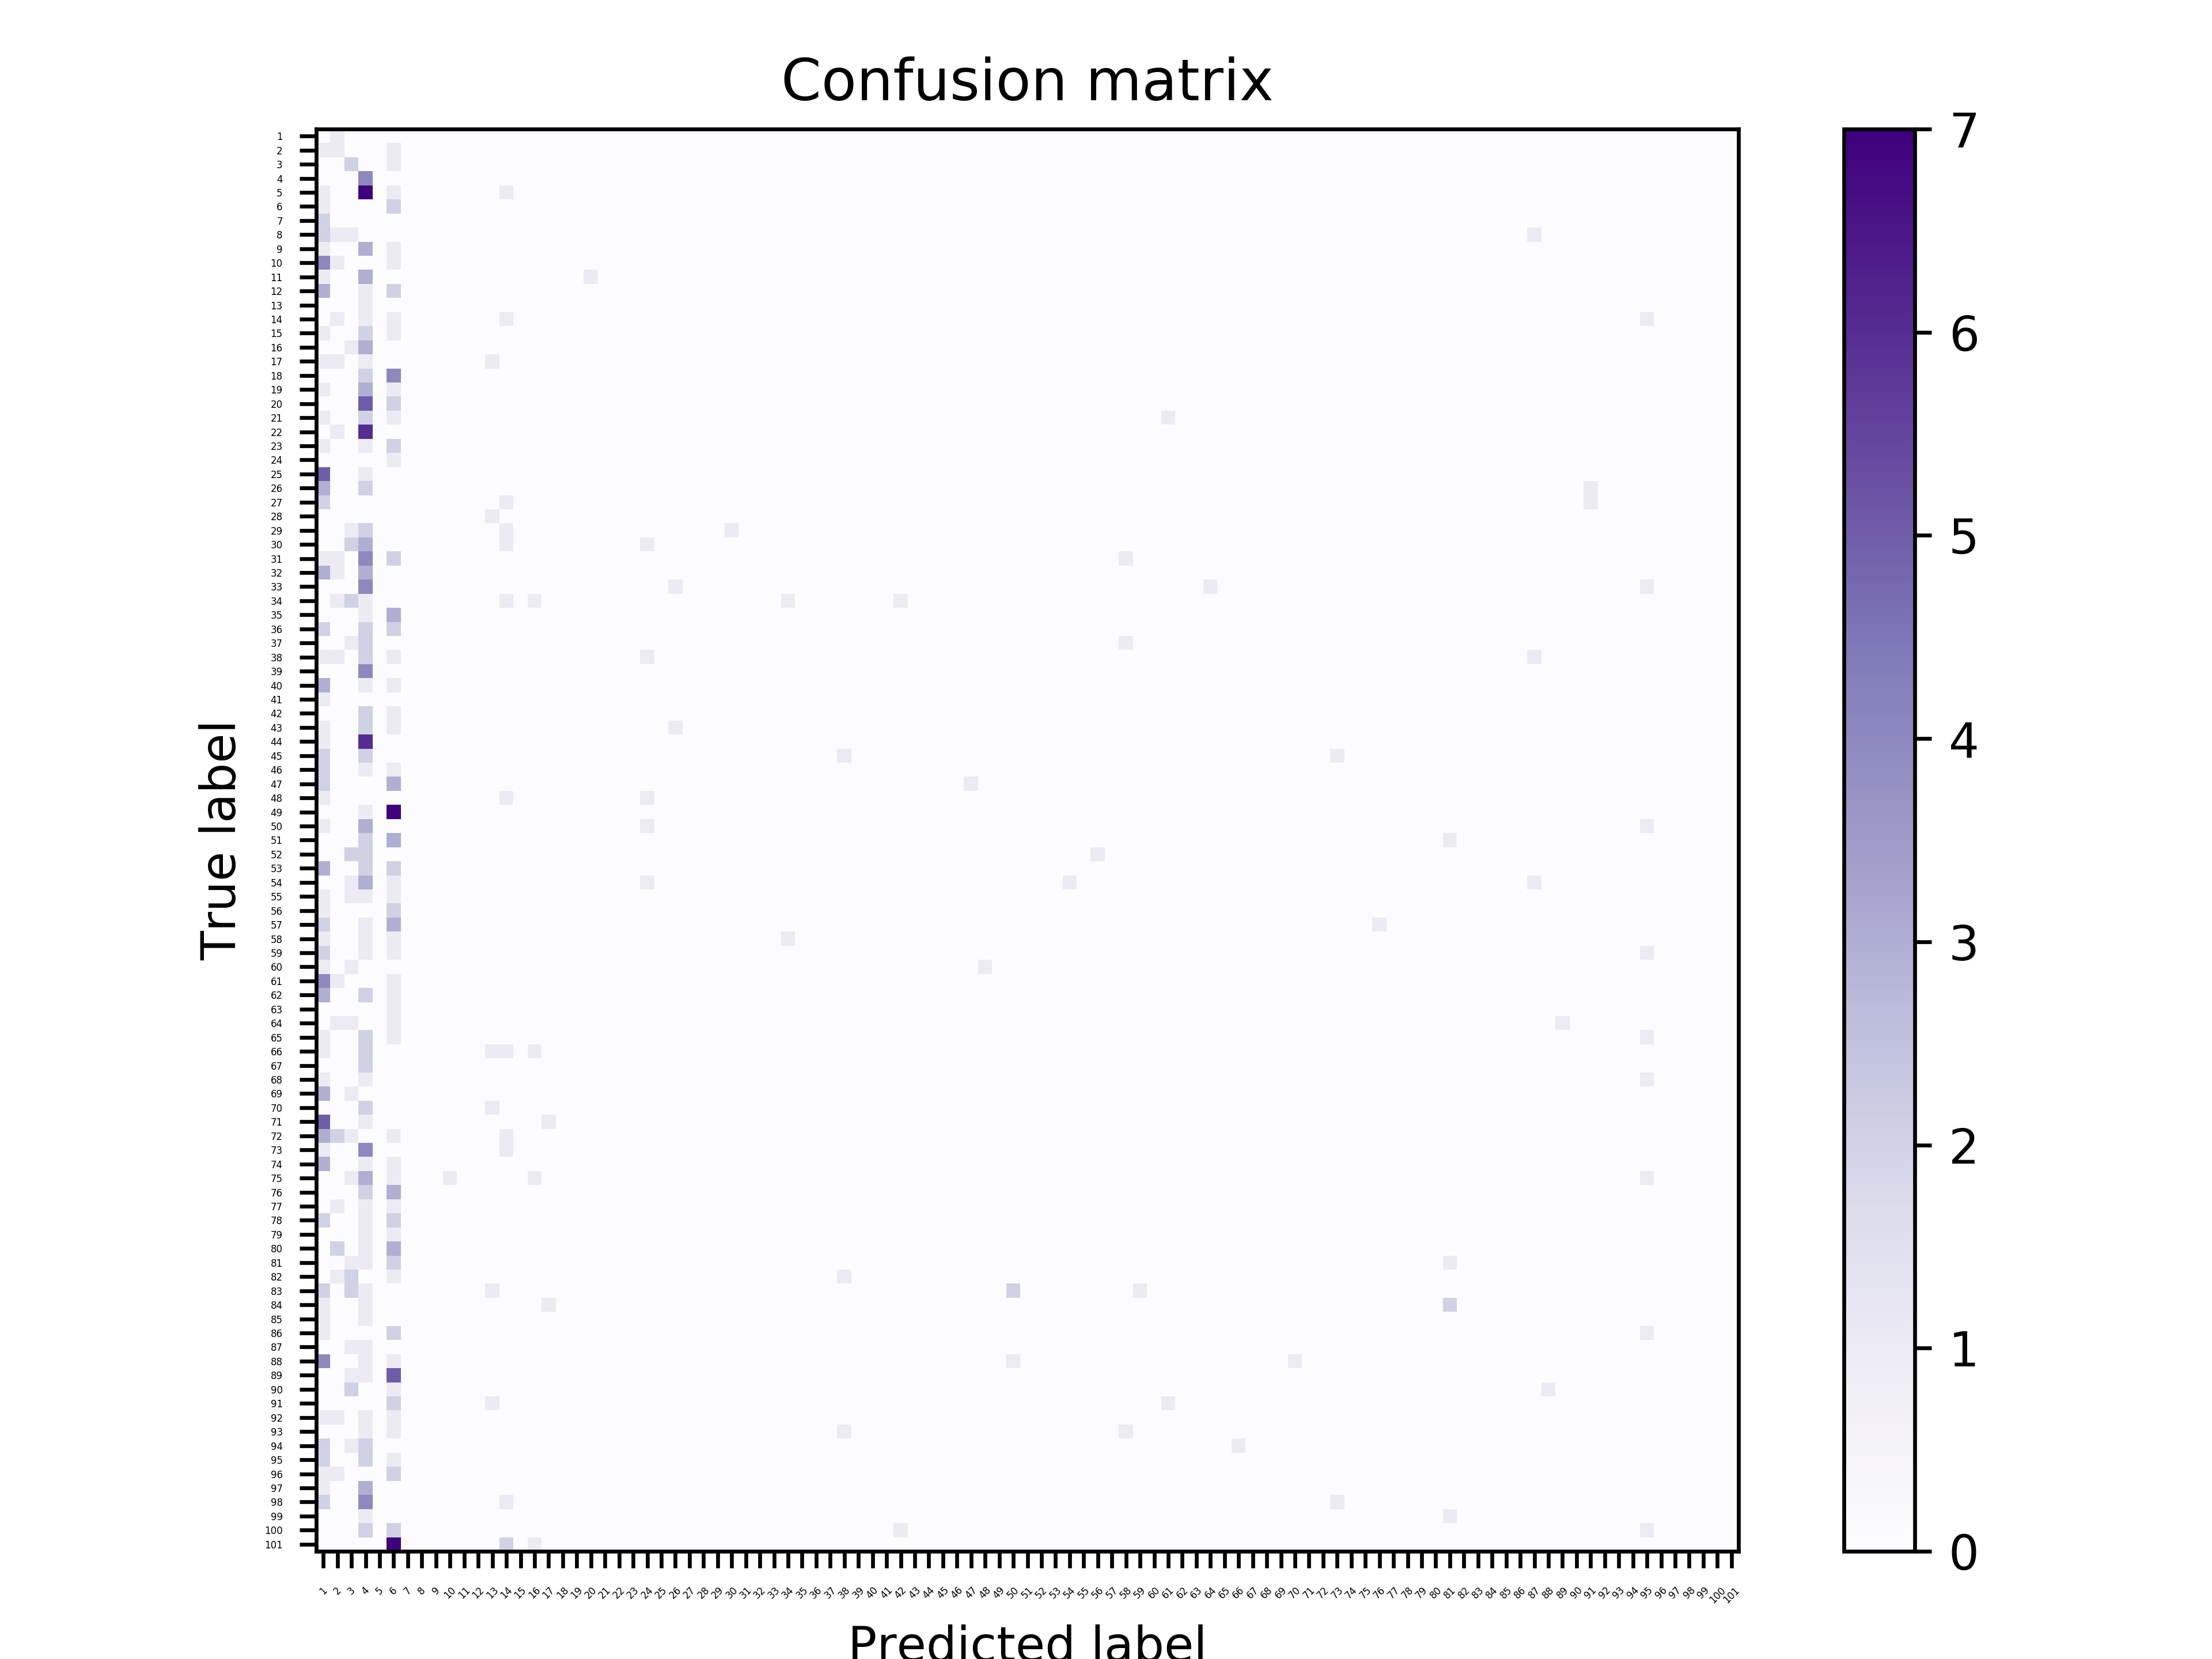
\includegraphics[scale=0.10]{bow_random_forest_confusion_results.jpg}


\subsection{Logistic Regression (Extra Credit)}

I train a logistic regression classifier provided via the scikit-learn library with default settings. My results give a $k$-fold cross validaton (on the training set, $k$ =5) average accuracy of 27\%. The logistic regression also gets about a 25\% training accuracy on the full training set. Finally, the test accuracy of this method is $1.6$\% accuracy. The confusion matrix is given below:

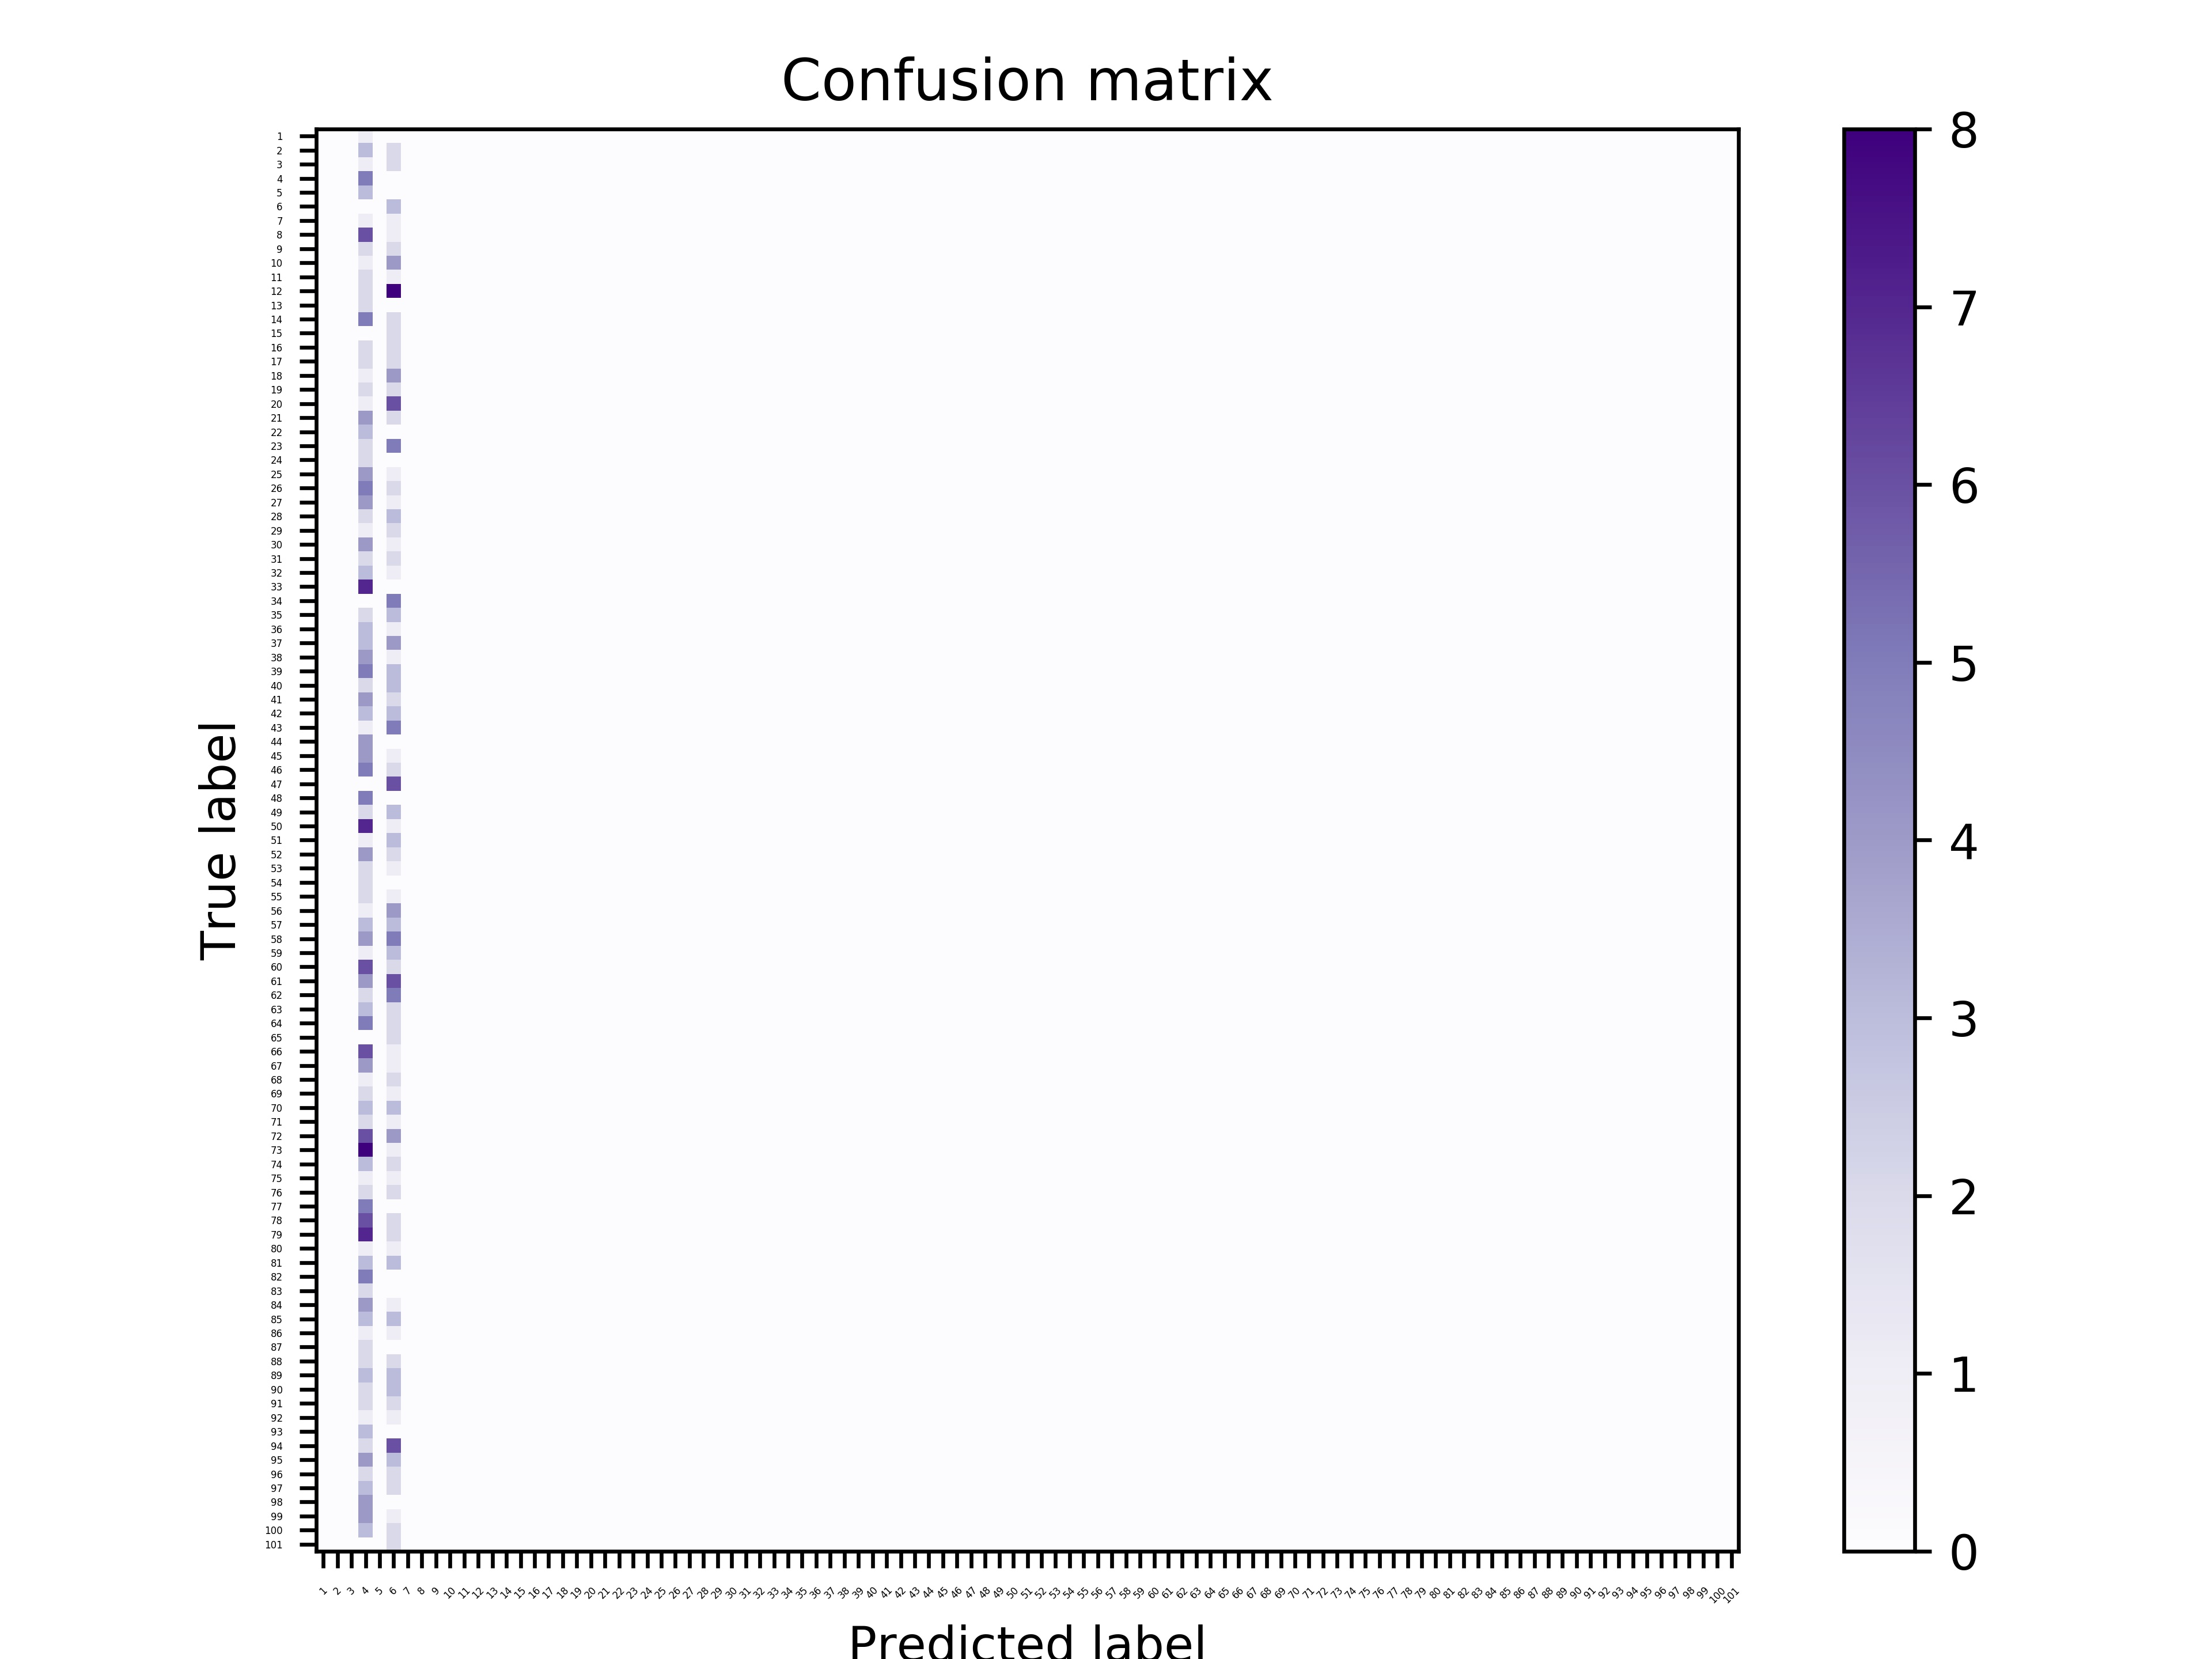
\includegraphics[scale=0.10]{bow_logistic_confusion_results.jpg}


\section{Alexnet}
Foor the alexnet implementation, I simply use the provided feature vector which is the output of a convolutional layer in the network.

\subsection{Random Forest}
I train a random forest with $n = 500$ decision stumps. The random forest achieves an average cross validation accuracy of $71$\% accuracy, while perfectly classifying the full training set, and achieves about $33$\% accuracy on the test set, which is vastly more impressive than the bag of words counterpart (although I did use a large number of estimators). 

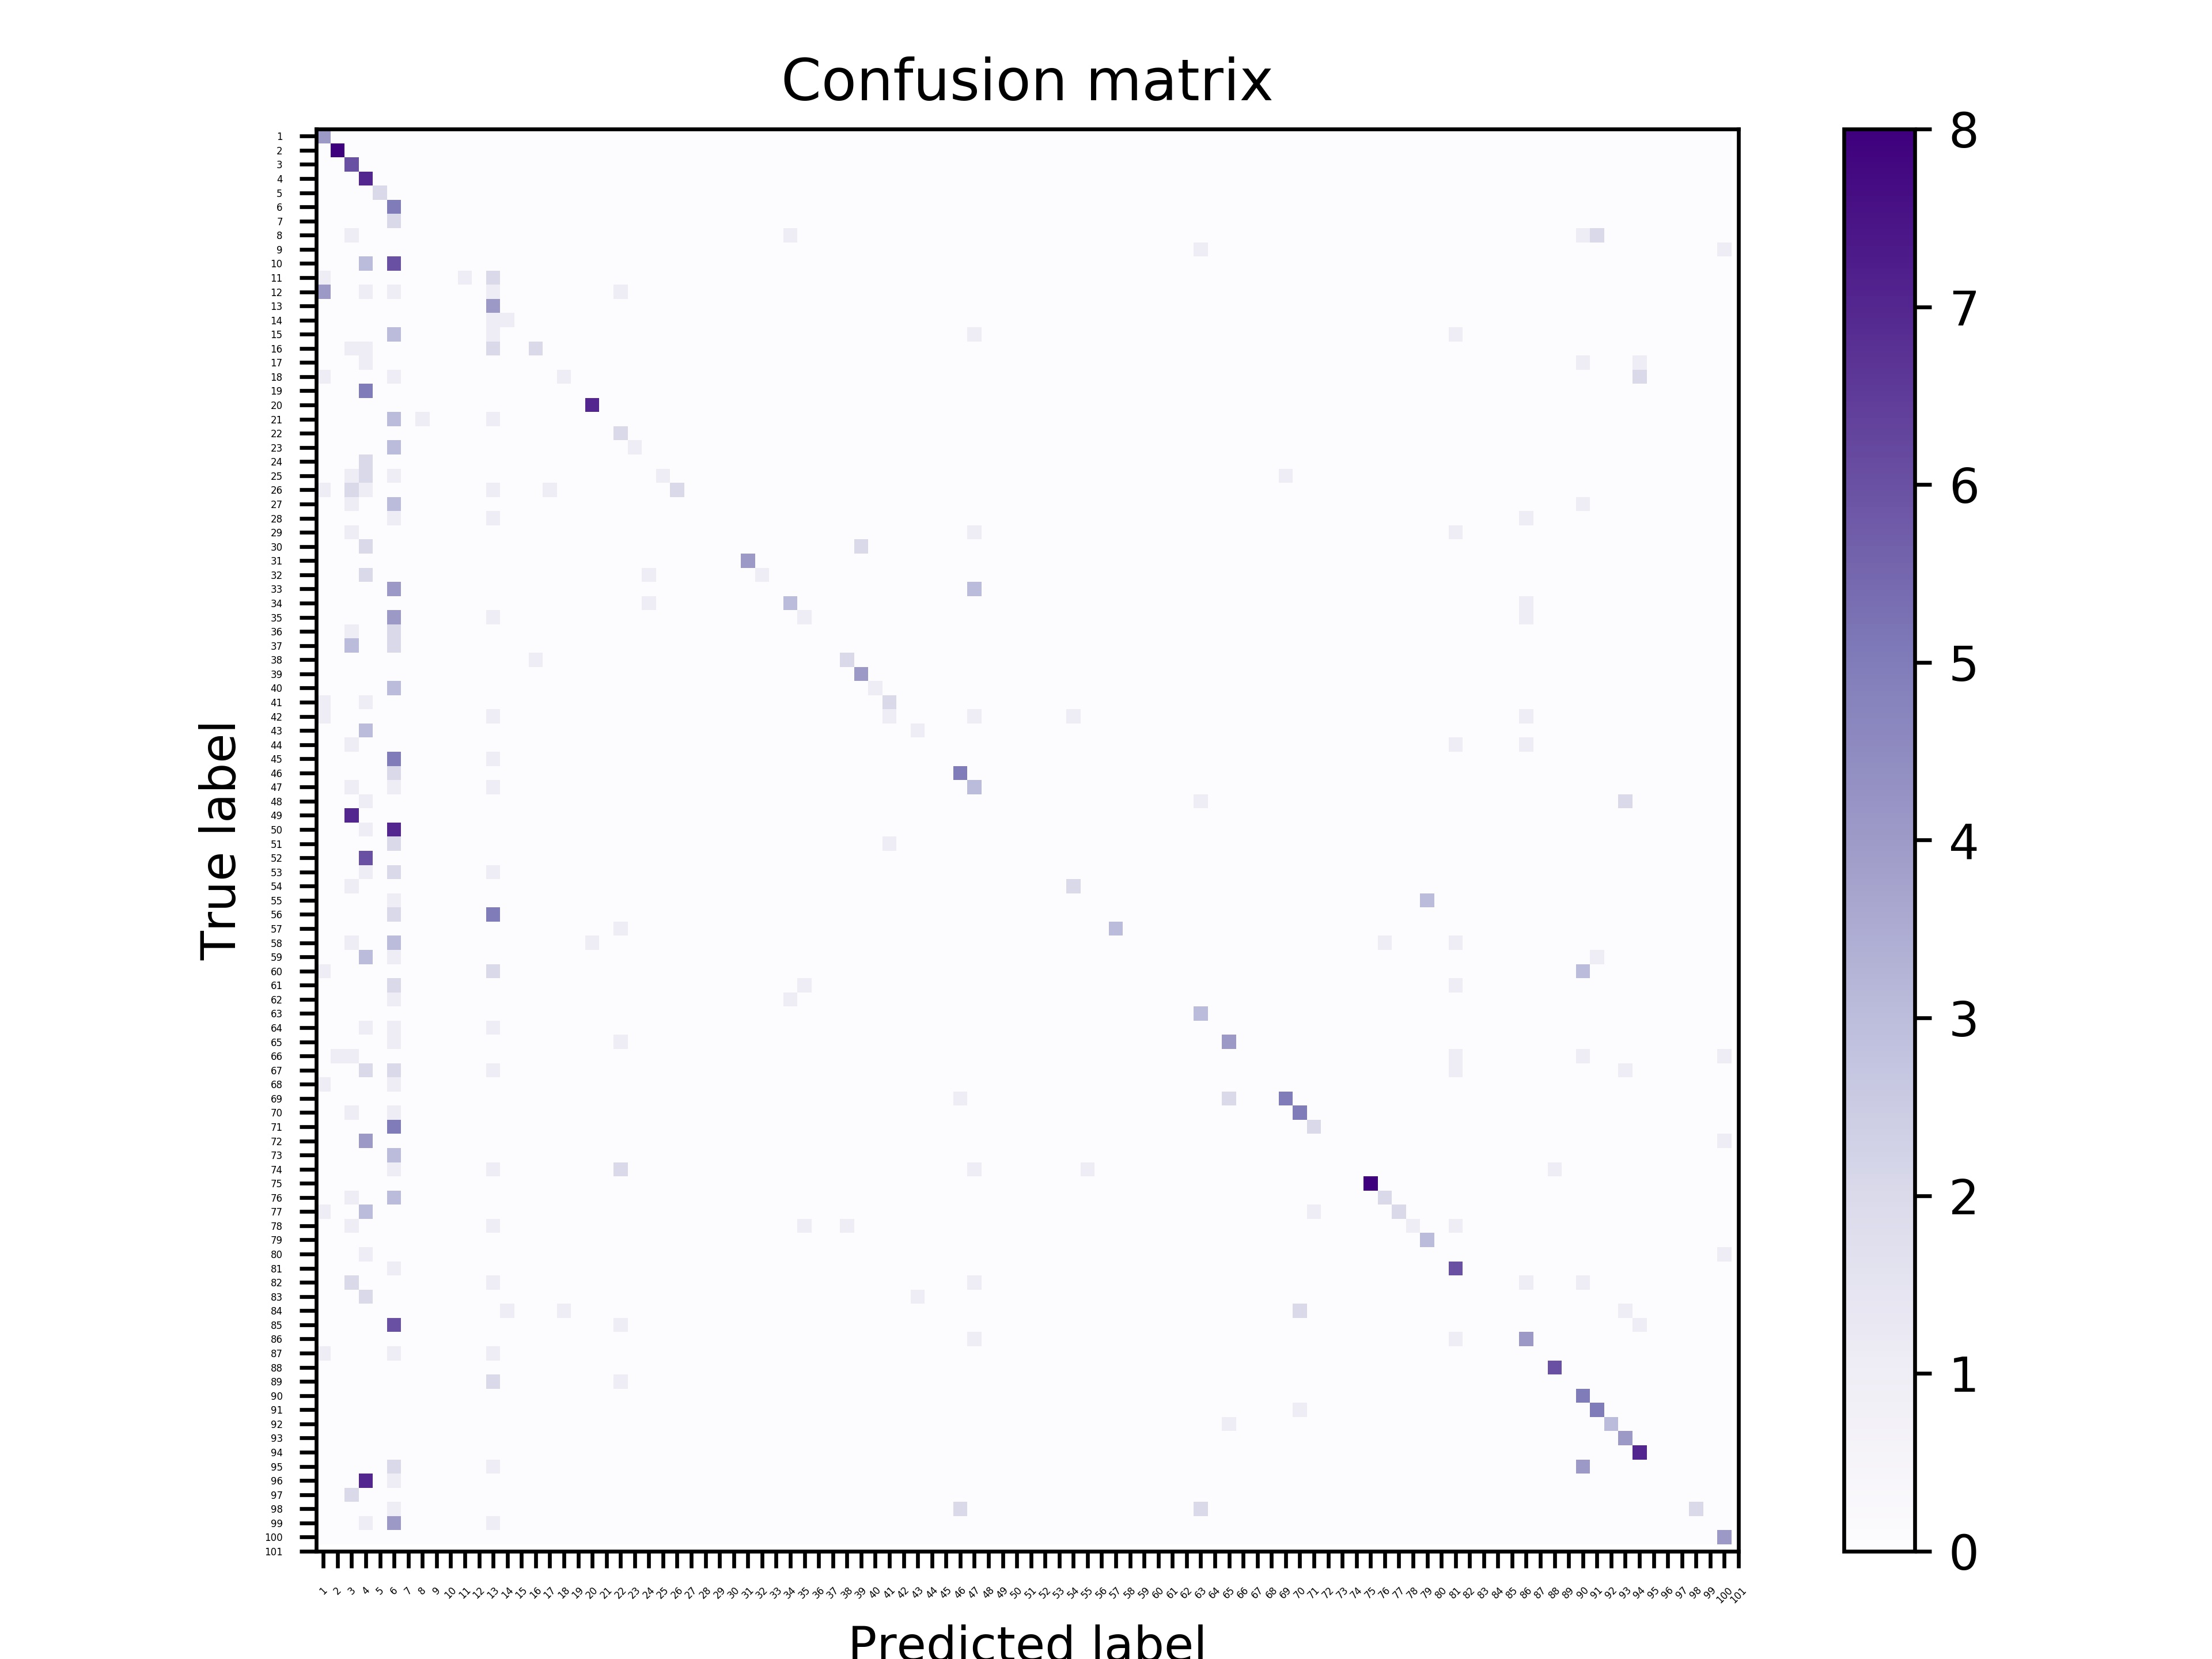
\includegraphics[scale=0.10]{alex_net_random_forest_confusion_results.jpg}


\subsection{Logistic Regression}
I train a logistic regression classifier with default parameters. The logistic classifier achieves an average cross validation accuracy of 81\% accuracy, perfectly classifies the full training set, and achieves a testing accuracy of approximately 57.6\% accuracy, by far the best result.

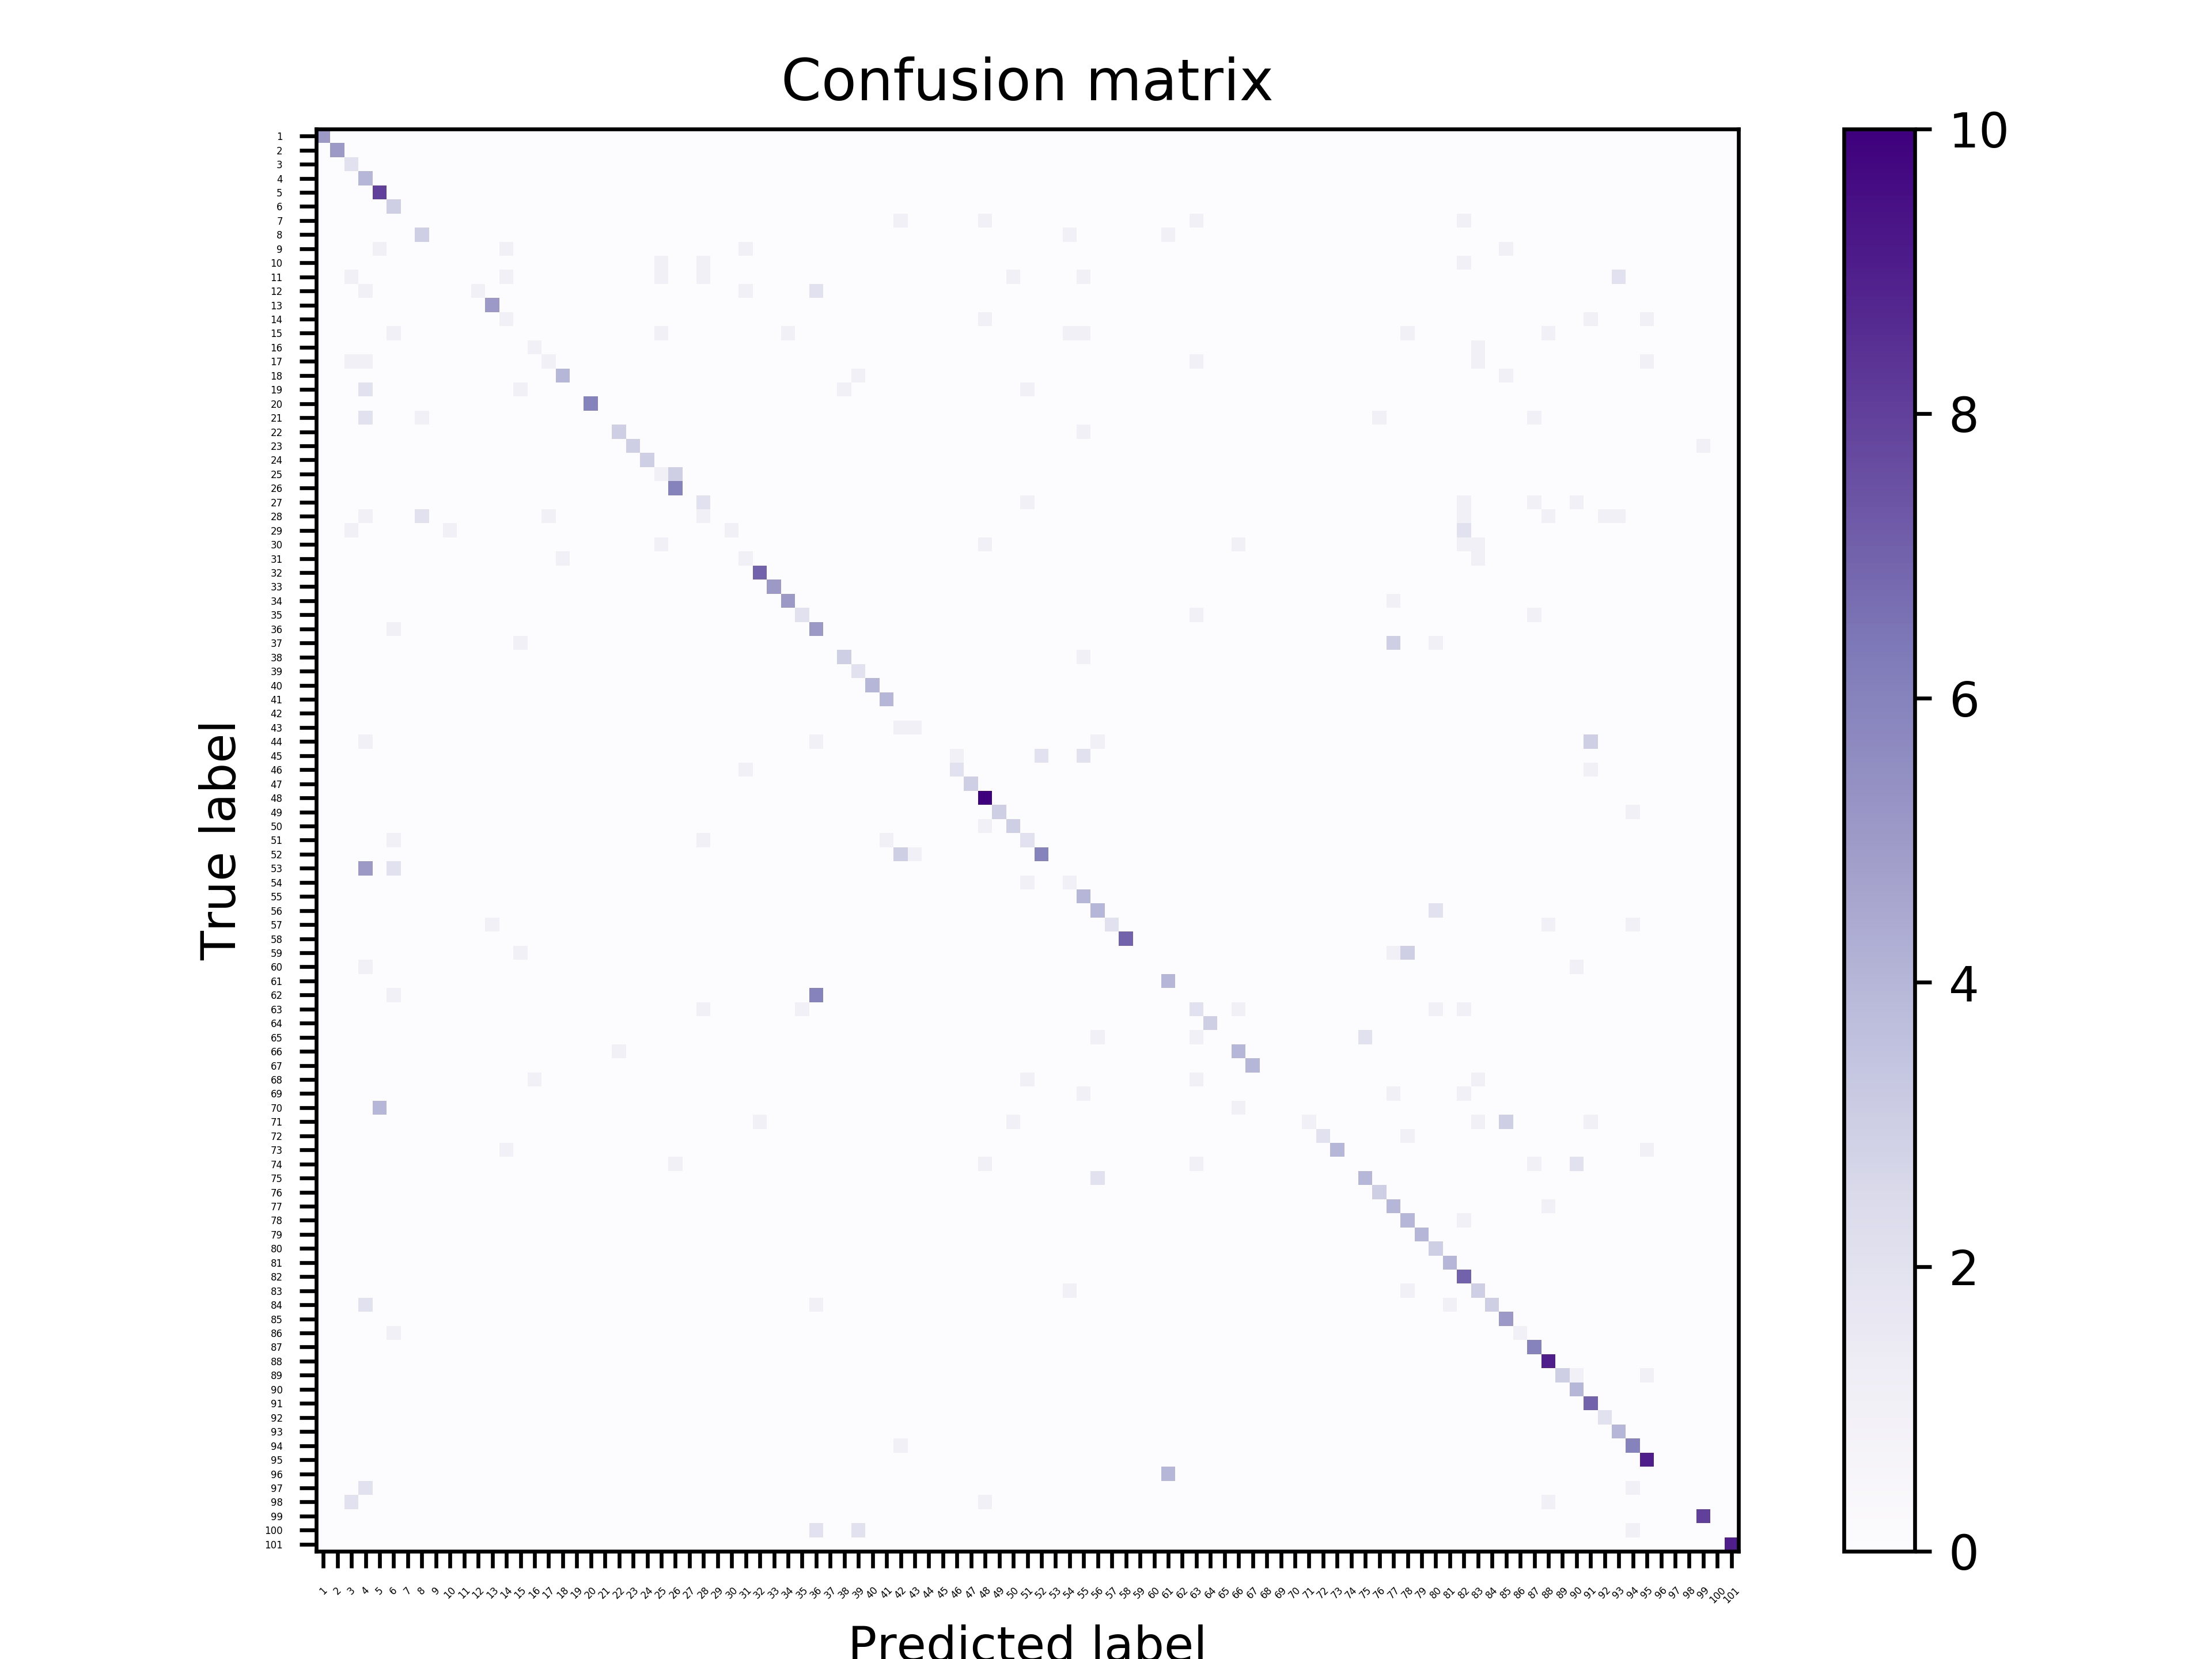
\includegraphics[scale=0.10]{alex_net_logistic_confusion_results.jpg}

\section{Conclusions}
Overall, I found the combination of a logistic regression classifier trained with AlexNet features to be the most accurate predictor of the image class. AlexNet is able to generate informative features that are perhaps better at incorporating global information better than the bag of words features, which is a local feature aggregation method. Moreover, logistic regession is a powerful classification tool that can fit many non-linear decision problems and be quite successful.

\end{document}